\documentclass[a4paper,UKenglish]{article}
\usepackage[utf8]{inputenc}
\usepackage{fontenc,url}
\usepackage{babel,textcomp}
\usepackage[round]{natbib}
\usepackage{graphicx}
\usepackage{subcaption}
\graphicspath{ {images/} }
%\usepackage{enumitem}
%\urlstyle{sf}

\title{DEM generation from optical satellite stereo}
\author{Kasper Skjegggestad}
\begin{document}
\maketitle
\tableofcontents

\section{Intro}

Digital elevation models (DEM), or digital terrain models (DTM) are widely used in research by scientists in governmental, university and private organizations. It is particularly useful for for geoscientific applications such as glaciers and rock-glaciers, geomorphology and georisk, hydrology, and land cover/ land use \citep{toutin08}. By analyzing DEMs you can, among other things, estimate were a landslide might originate, estimate precipitations zones or estimate the volume changes of a glacier. All researches based on DEMs will be dependent on the quality of the DEM. The quality of a DEM depends on the method of how it was collected and generated. DEM can be generated with inSAR, LiDAR, and with stereoscopy. The last method will be discussed here, and are based on Thierry Toutin papers from 2001 (Elevation modelling from satellite visible and infrared (VIR) data) and 2008 (ASTER DEMs for geomatic and geoscientific applications: a review).

\section{Generating DEM}
Everything we see is in 3D, this is thanks to the fact that we have 2 eyes that catches the lightwaves from the objects we observe from two slightly different positions. Knowing this, we can create 3D images with the help of 2 cameras, or by taking a picture of an object or scene from two slightly different positions. It is these principles that helps us create DEMs from optical satellite stereo. The difference/parallax between the two images will help us find the elevation of an object. In principle, we have 2 methods of achieving stereo photo with satellites. Across-track stereoscopy from two different orbits, and along-track stereoscopy from the same orbit with one down-looking sensor (NADIR) and one back-looking or front-looking sensor (figure \ref{alongtrack}). The across-track stereoscopy will have photos taken on different dates, while the along-track stereoscopy images are acquired withins seconds apart from each other. This makes the images more similar to each other (e.i. same lighting), and therefor more suited for image matching.

\begin{figure}
	\centering
	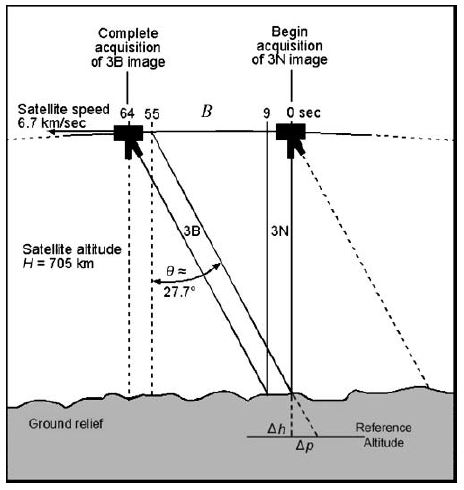
\includegraphics[height=12.5cm]{alongtrackfigure}
	\caption{Alongtrack satelite \citep{toutin08}}
	\label{alongtrack}
\end{figure}

\cite{toutin01} describes the different processing steps to produce DEMS from stereo images in the following terms: 

\begin{enumerate}
	\item acquire the stereo image data with supplementary information such as ephemeris and attitude data if availeble;
	\item collect Global Control Points (GCP) to compute or refine the stereo-model geometry;
	\item extract the elevation parallax;
	\item compute the 3D cartographic co-ordinates using 3D stereo-intersection; and
	\item create and post-process the DEM (filtering, 3D editing and smoothing).
\end{enumerate}

\subsection{Acquiring data}

 ASTER (Advanced Spaceborne Thermal Emission and Reflection Radiometer) is a satellite with both a downward looking sensor, and a backwards looking sensor. ASTER was sent up to obtain high spatial resolution of the earth. The objectives of ASTERs along-track stereo experiment were; to acquire cloud free stereo coverage of 80$\%$ of the Earth' land surface between 82$^{\circ}$N and 82$^{\circ}$S, and to produce, with commercial software, standard product DEMs at a rate of one per day \citep{toutin08}. Due to the high temporal resolution provided from ASTER, i's stereo photos are now one of the most used in DEM generation. There are several commercial of the shelf (COTS) softwares for processing stereo ASTER data and for generating DEMS, such as PCI Geomatica and silcAst. ASTER produces two types of data, level 1A and level 1B. Level 1A is the preferred data by photogrammetrist. Level 1A consists of the raw image with only detector normalization and calibration. Level 1B is a geo-referenced image corrected for the systematic distortions due to the sensor, the platform and the Earth rotating and curvature \citep{toutin01}. 

 ASTER provides stereo images of high spacial resolution. And since it creates along-track stereo images, they are well suited for image matching. Image matching is important to find the parallax of objects in the two different photos.The process to extract elevation parallax is applied using the image grey-levels, the image features or a hybrid appoach \citep{toutin08}. 

\subsection{Global Control Points}
After the stereo image is acquired, GCPs should be collected. GCPs are collected in order to obtain a cartographic standard accuracy. They are collected by finding a point in both image were you know the coordinates and/or elevation. The GCPs should cover the full elevation range of the terrain, and to avoid extrapolation in planimetry, it should be spread at the border of the stereo-pair. \cite{toutin01} mentions three different types of GCPs that can be used:
\begin{itemize}
	\item full control points with known XYZ co-ordinates;
	\item altimetric points with known Z co-ordinates; and
	\item tie points with unknown cartographic co-ordinates.
\end{itemize}
Tie points and points with known Z co-ordinates are useful to fill in gaps where no XYZ GCP are placed, and they can reinforce the stereo geometry. GCPs that are on only one of the images, whether that is because the point was not found in one image, or the point is outside the boarder of one image, can be used as complementary points to the stereo GCPs. They will also be helpful to avoid extrapolation in planimetry in areas where there are no stereo GCP when combined with tie points \citep{toutin01}.

It is the GCPs cartographic and the images co-ordinates that mainly control the the final accuracy of the stereo geometry. There are several ways of acquire the GCPs cartographic data. Some examples are GPS, air photo surveys, paper or digital maps, previously ortho-rectified images or chip database. The accuracy of the GCPs will depend on the accuracy of whichever method was used in other to collect them, and in extend affect the stereo model reconstruction and the final product. When GCPs are collected with high uncertainty, it is recommended to increase the minimum number of GCPs \citep{toutin01}.

\subsection{extraction of the elevation parallax}

The elevation parallax can be extracted using image matching with two methods. Ether by computer-assisted(visual), or automatic methods. It is possible to integrate these two methods in order to get the strength of each one. With the computer-assisted method, a computer screen using a system of optics is used to realize the stereoscopic viewing. For spatial separated stereo images, two monitors or a split screen are used with an optical system using mirror and/or convex lenses \citep{toutin01}.


\subsection{Post-processing the DEM}

When the DEM is extracted from the stereo images, some post-processing will be necessary. Witch process that will be necessary, depends on the quality of the DEM and the method it was extracted with. post-processes can help to (among other things) remove blunders, fill mismatched areas and smoothen the DEM. When there are big differences between a value and its neighbors, a blunder removal function is needed. A blunder removal function use filters based on statistical computations like mean and standard deviation. Good elevation values can be used with interpolation to fill mismatched and noisy areas. Filtering can be used in order to remove pits and hummocks, but it should preserve sharp breaks in slopes. Filtering may improve the relative DEM accuracy or the relationship between neighboring values, but the DEM accuracy will be determined by the generation method, system and software \citep{toutin01}.


\section{Conclution}

ASTER provides high temperoal stereo images. With theres, there are good posibilityes to generate DEMs over most of the world. COTS softwares like PCI geomatica and silcAst makes it easyer for end users to create a DEM over their desired area. After the stereo images and the GCPs are collected, PCI Geomatica and silcAst can do the rest of the steps for you more or less automatic (allowing you to choose and alternate some paramteres). SilcAst does not even require GCPs. SilcAst was developed exclusively for ASTER. There are, however,  no information on the algorithms in their web side or in the public literature. Of all the DEMs analyzed by \cite{toutin08}, the DEM from silcAst achieves the lowest root mean square error of 6.1, even without the use of GCPs.

The end users still have to be aware of biases in the DEM they create, and checking the accuracy of your DEM is highly advised. Post-processing the product can improve the DEM, fill inn areas with no data, and smoothen the DEM

\bibliographystyle{apalike}
\bibliography{kilder}

\end{document}
